\section{Experiments}

In order to properly study and select the different configurations, it is
necessary to analyize the behaviour of the algorithm, when we modify one
parameter at a
time. An automated test was developed for this purpose, provided in the annex,
with which we run a set of tests, changing the number of individuals, the number of
generations, the percentage of elitism, and the balance of percentage of
mutation and crossover. Each test, in each city is run a total of 5 times,
and the average is what is taken into account. \\
After that, a set of tests, created from the results obtained in the general
set, is made, by selecting specific values. Both the general, and the specific
tests will serve as a medium to compare both representations, in order to look
for differences (or lack thereof)
\\
For the general tests, the default values are:\\
\\
\begin{itemize}
  \item Number of individuals - 50
  \item Number of generations - 50
  \item Elitism - 0.05
  \item Crossover - 0.95
  \item Mutation - 0.05
  \item Stop percentage condition - 0.95
  \item Detection of loops on
\end{itemize}
\\
And, the different values for each modified parameter are
\begin{itemize}
  \item Number of individuals - [50,100,150,200,500,750,1000]\\
  \item Number of individuals - [50,100,150,200,500,750,1000]\\
  \item Elitism percentage - [0,0.05,0.1,0.2,0.5,0.75,1]\\
  \item Crossover|Mutation balance - [1|0,0.95|0.05,0.9|0.1,0.75|0.25,
0.5|0.5,0.25|0.75,0|1]\\
\end {itemize}
\subsection{Adjacency representation}
\\
With the provided representation, adjacency representation, the results of the
general tests are:\\
\\
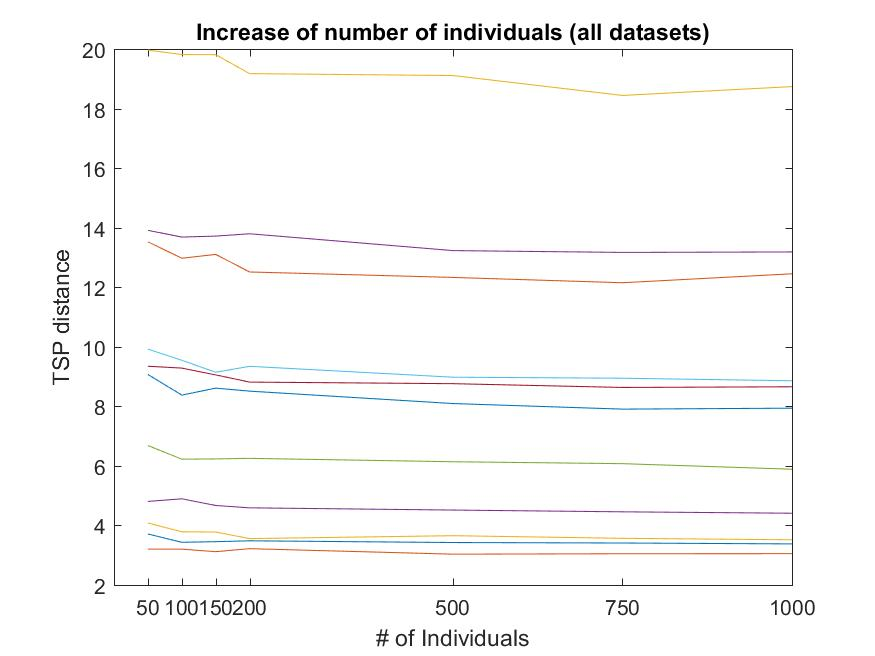
\includegraphics[width=\textwidth]{img/xalt_edges/numberIndiv.jpg}\\
As expected, a relatively low number of individuals does not provide adecuate
results, as can be observed by looking at the start of the graph. Almost
all datasets start in global maximum, and only a couple in a local max. However,
the mayority of them have one of their lowest point when the number of
individuals is 200 (except for the highest dataset, which has it's lowest
point at 750) and from that point, it stays constant, or even raises, as
happens with the highest, and third highest dataset, thus it can be said
that any number of individuals higher than 200 would not be benefitial, and
actually be just cumbersome when it comes to computational cost. 
\\
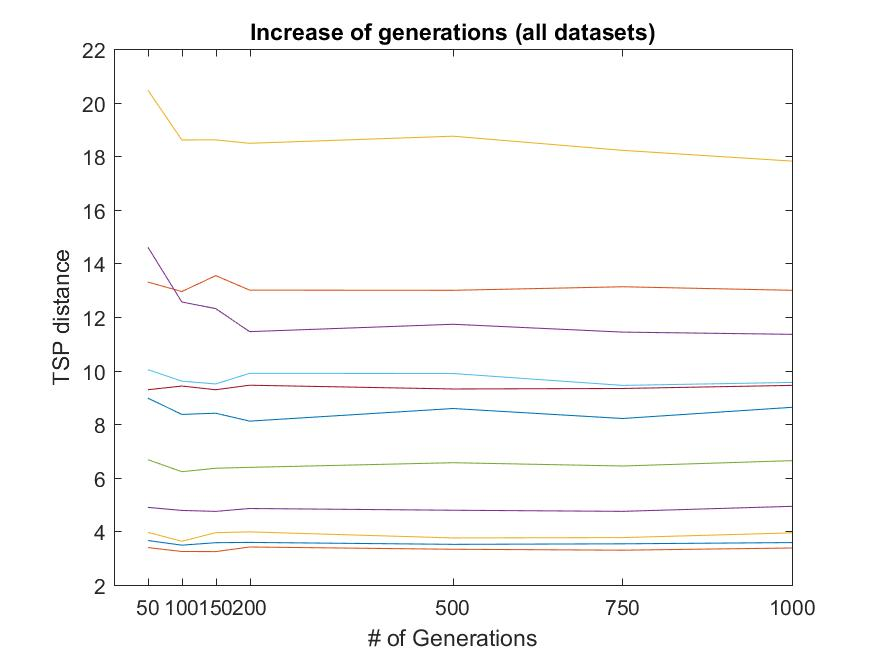
\includegraphics[width=\textwidth]{img/xalt_edges/numberGens.jpg}\\
Once again, it is to be expected that a low quantity of generations will not
yield good results. But that is not the only thing the number of
individuals and generations have in common, since it seems like 200 is one of
the best options for the number of generations. There are some
differences, for instance, at lower quantities of generations, there is more
fluctuation, and more datasets are positive towards higher number of
generations. In the specific tests this will be further studied, whether
200, or a higher number is better, and whether the higher
associated computational cost is worth.
 \\

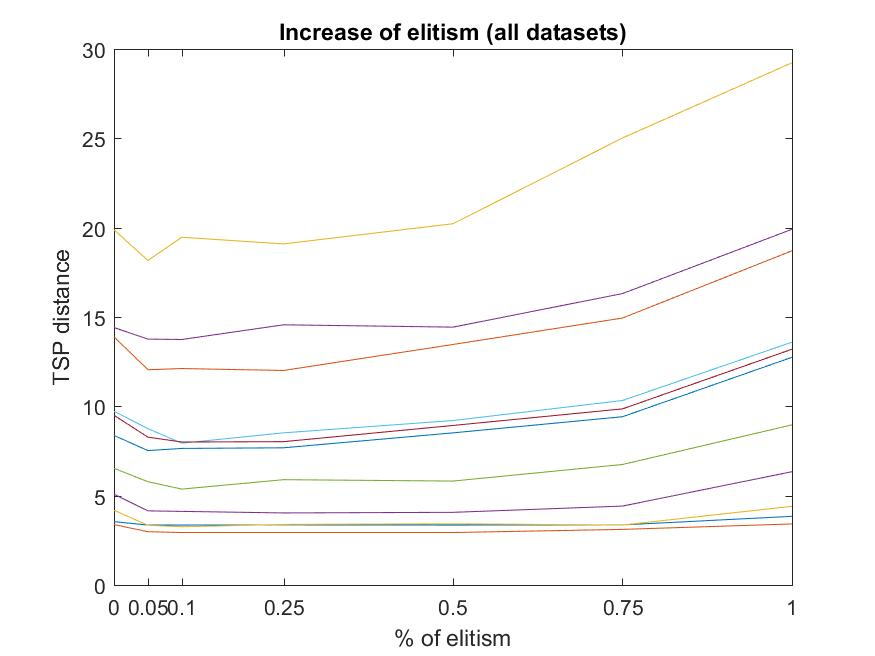
\includegraphics[width=\textwidth]{img/xalt_edges/elitism.jpg}\\
When it comes to the percentage of elitism, the results are much more clear.
With no exceptions, the lowest value for every single one of the datasets
is between 0.05 and 0.1, any higher, or any lower, and the distance
skyrockets, having the highest distances values at elitism = 1. \\
This phenomena has an easy explanation, the higher the elitism, the more likely it is that the
algorithm will stay at a local maxima. \\


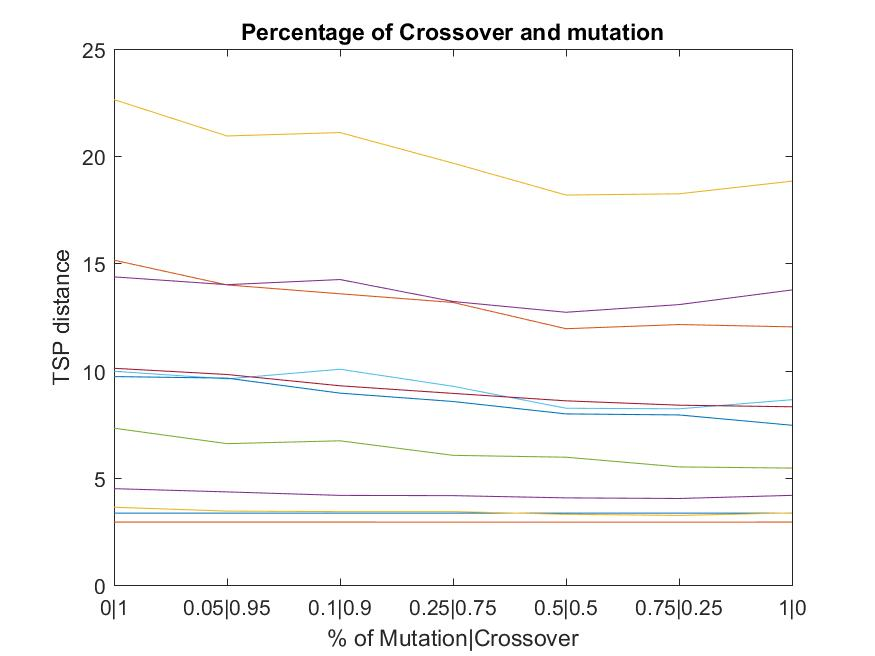
\includegraphics[width=\textwidth]{img/xalt_edges/crossMut.jpg}\\
The test reflects perfectly the balance between exploitation and
exploration, the overall result shows that the best performance comes when
mutation has a value of 0.5, and crossover 0.5.\\
Any value of mutation higher than 0.5, and the results start to worsen, because
there is too much exploitation, and too litle exploration. Any value of mutation
lower than 0.5, and the results, most of the cases, are far worse. This leads to
the conclusion that 0.5 is the candidate for the specific tests, alghouth
the nature of the result makes it necessary to test other values, since,
\textcolor{red}{we think these results are a bit odd, hence we will further
study in the specific tests, order to make a conclussion}


\subsection{Path representation}\\
As explained in the implementation section, the representation we
implemented is path representation. The results after executing the same
tests as before are\\
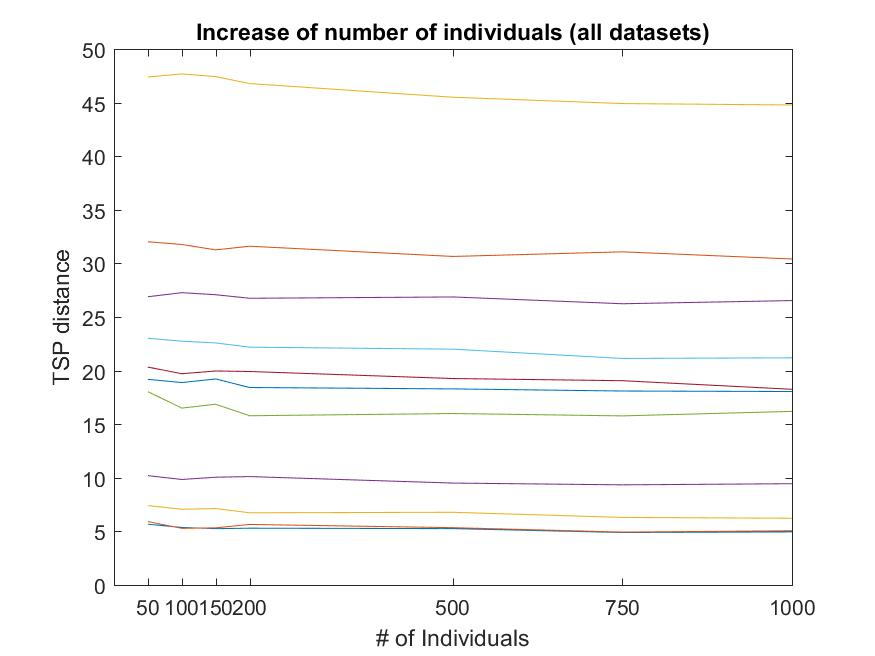
\includegraphics[width=\textwidth]{img/order_crossover/numberIndiv.jpg}\\
Similarly to adjacency representation, the result for the test
of increasing the number of individuals has a generally located minimum local at
200, although for some cases, the distance becomes constant at 100. The only
noticeable difference is that it is more stable at lower quantities of
individuals, and the values for the distances when the number of
individuals is very high (750,100) does not increase, rather it seems to keep
ever so slightly decreasing. \\
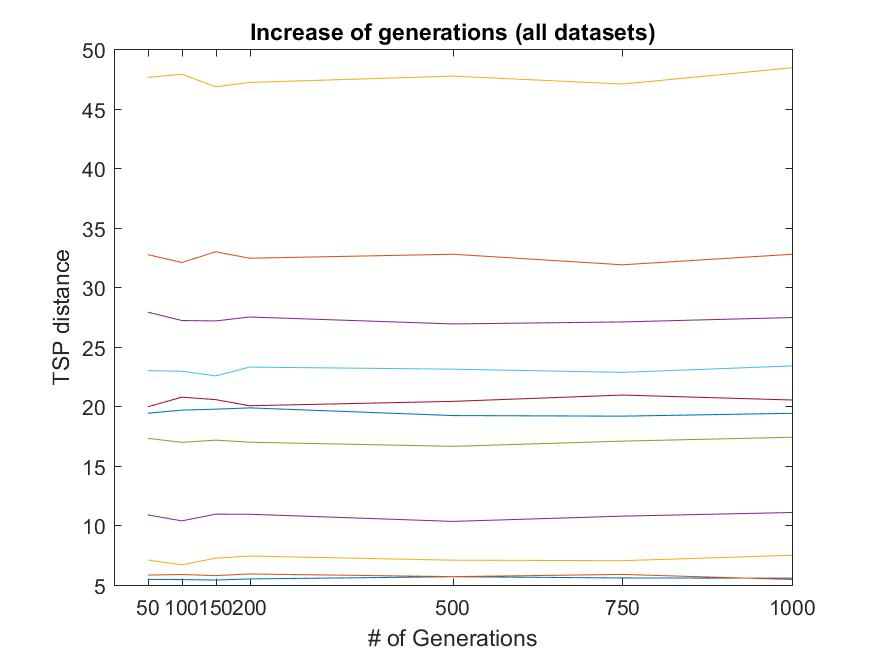
\includegraphics[width=\textwidth]{img/order_crossover/numberGens.jpg}\\
Once again, as expected, there is a number of individuals from which the
change in the result is null. That point, as can be observed, is 200
individuals, the same as the other representation. But then again, there
are differences, two main ones, the first, the change from 50 to 100
individuals is not so apparent, and the values obtained from 750
individuals forward is actually worse in some cases, if not the same, while
with the other representation there were some cases in which it
improved. \\
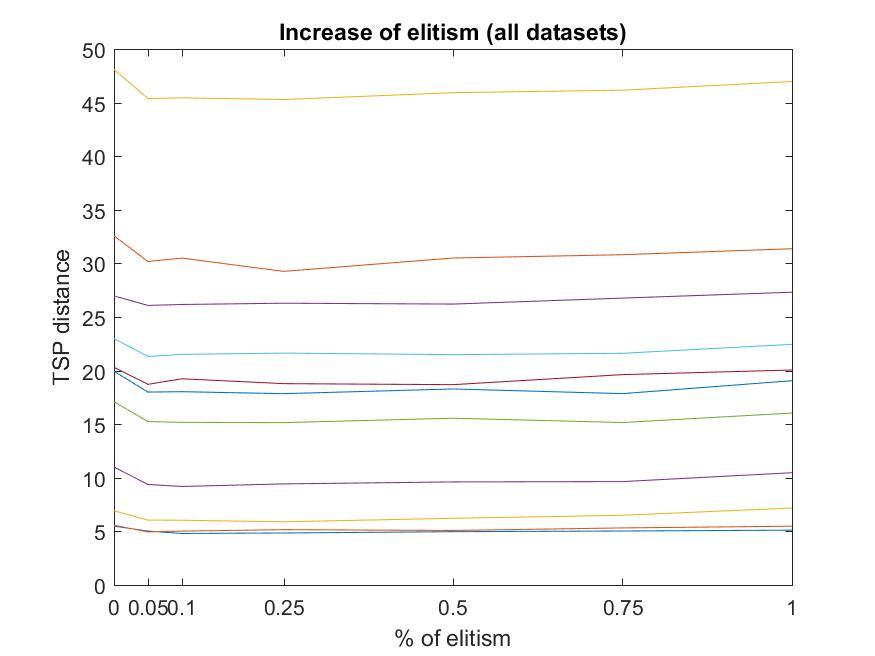
\includegraphics[width=\textwidth]{img/order_crossover/elitism.jpg}\\
From what can be observed, there is no doubt that 0.05 is the best
percentage of elitism that can be choosen with this representation. The results
are somewhat similar to the previous representation, but the slope at the
latest values (0.5 forward) is not so steep\\
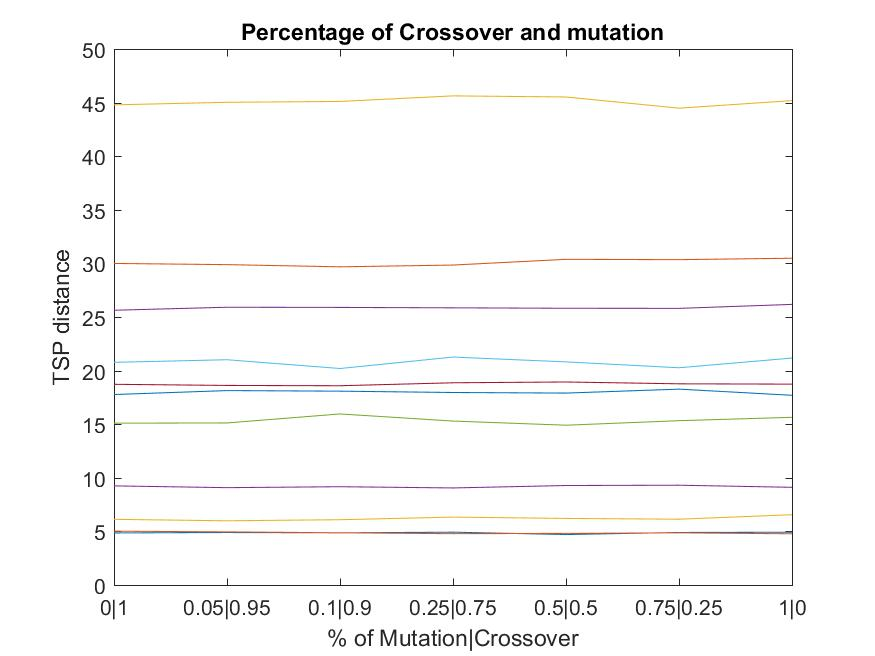
\includegraphics[width=\textwidth]{img/order_crossover/crossMut.jpg}\\
The result of this test is daunting. It was repeated, in case it was somehow
erroneous, but the same graph was obtained. With our representation, there
seems to be no effect whatsoever on the exploitation vs exploration dilemma.
\textcolor{red}{It does not matter, apparently, the percentage of mutation
or crossover}
\\


\subsection{Specific tests}


